%% LyX 2.0.3 created this file.  For more info, see http://www.lyx.org/.
%% Do not edit unless you really know what you are doing.
\documentclass[english]{article}
\usepackage{mathptmx}
\usepackage{helvet}
\usepackage{courier}
\usepackage[T1]{fontenc}
\usepackage[latin9]{inputenc}
\usepackage{geometry}
\geometry{verbose,tmargin=2.54cm,bmargin=2.54cm,lmargin=2.54cm,rmargin=2.54cm}
\usepackage{graphicx}
\usepackage{babel}
\begin{document}

\title{Finding conserved transcription factor binding sites by comparing
ChIP-seq experiments}


\author{Colin Diesh}


\date{Senior Thesis Project, Fall 2012\\
$\,$\\
First semester final report}
\maketitle
\begin{abstract}
DNA-protein interactions are essential for gene regulation, and these
interactions can be detected by using chromatin immunoprecipitation
and high throughput sequencing (ChIP-seq). Transcription factors in
particular are proteins that bind to specific sequences on the DNA,
thereby promoting or suppressing the transcription of nearby genes.
Using ChIP-seq, transcription factor binding sites are identified
as peaks in the data that represents a \textquoteleft{}tag pileup\textquoteright{}
of DNA sequences. Some binding sites have too weak of a signal to
confidently identify, but evidence from comparing ChIP-seq experiments
from the genomes of related strains may provide the additional support
needed to identify these. We found substantial evidence for weak binding
sites that are conserved but aren\textquoteright{}t found by other
peak finding algorithms, and we use a normalized difference score
described by Zheng et al (2010) to find some of these. We also introduce
a modified normalized difference score that uses data from multiple
genomes concurrently.
\end{abstract}

\section{Introduction}

The genes in our DNA are regulated by a variety of proteins that interact
and bind with the DNA. Transcription factors in particular are proteins
that can affect DNA transcription by binding to the DNA, thereby regulating
nearby genes. Transcription factors bind to a particular DNA motif,
which is a short DNA sequence that they are attracted to. Identifying
the transcription factor binding sites has become an important problem
for understanding gene regulation. However, comparisons of different
related species have shown a high degree of variability of binding
sites in human and mouse and in different strains of yeast (Odom et
al. 2003, Zheng et al. 2010). 

ChIP-seq is a next-generation sequencing method for detecting DNA-protein
interactions. ChIP-seq uses chromatin immunoprecipitation followed
by high throughput sequencing to find DNA sequences to which transcription
factors bind. ChIP-seq data is made up of many short DNA sequences,
and after the sequences are aligned to a reference genome, the transcription
factor binding sites appear as \textquoteleft{}peaks\textquoteright{}
in the data. Peak finding algorithms use a significance level that
is based on a somewhat arbitrary threshold. 

In order to compare ChIP-seq data, typically, the binding sites from
different experiments are identified from each experiment individually,
and if the location of a binding sites overlap at the same genome
position in each experiment, then they are shared. If the comparison
involves comparing different genomes, then we can either compare nearby
genes of the binding sites if there exist homologous genes to compare.
Other techniques for comparing binding sites from different genomes
use a DNA alignment of each genome to find overlapping binding sites.
Odom et al. (2007) developed a peak classification that uses DNA alignment
and the ChIP signal to compare human and mouse binding sites which
illustrates how binding sites can vary from comparing different genomes.

Using the peak classification, conserved binding sites are defined
as binding sites that have the same target gene which also have conserved
DNA alignments. The conserved DNA alignment is typically characterized
using motif finding (Odom et al. 2007) but they can also use multiple
sequence alignments (Moses et al. 2004). A gained or lost peak will
have conserved sequences, but they will not have similar peak characteristics.
The unaligned and turnover classes of peaks will not have a matching
the sequence alignment, \textquotedblleft{}so they can not be classified
definitely\textquotedblright{} (Odom et al. 2007).

\begin{figure}


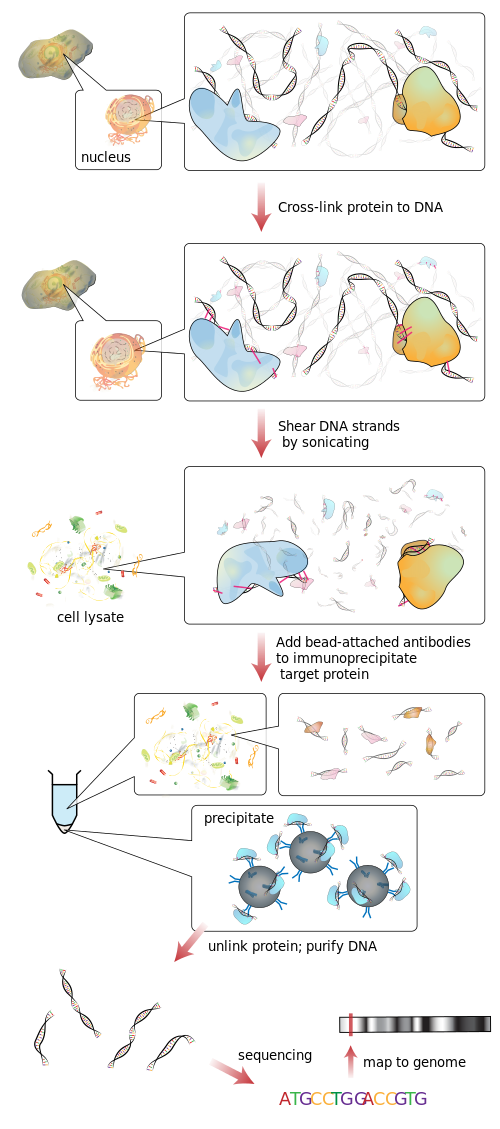
\includegraphics[scale=0.6]{image1}

\caption{Peak classification uses a DNA alignment to classify identified binding
sites (Odom, Dowell et al, 2007)}


\end{figure}


Some binding sites have too weak of a signal to confidently identify,
but evidence from the genomes of related strains may provide the additional
support needed to identify these. Using the normalized difference
score (NormDiff) described by Zheng et al (2010), we were able to
find substantial evidence for conserved binding sites that were not
identified by MACS, a commonly-used tool for identifying binding sites
from ChIP-seq data, by comparing the NormDiff scores from peaks identified
in one experiment with the same region from another experiment (the
syntenic region). We were able to identify some additional peaks found
in one strain as conserved with a statistical analysis of the NormDiff
values. We also present modifications to the normalized difference
score that use the data from multiple genomes concurrently.


\section{Background}


\subsection{Genetic analysis of transcription factor binding variation in yeast
(Zheng et al. 2010)}

In 2010, Zheng et al. analyzed transcription factor binding sites
in two strains of yeast, S96 and HS959, by using ChIP-seq for a transcription
factor called Ste12. They found transcription factor binding sites
using MACS software (section 2.2, appendix A). About 40\% of the binding
sites are found to vary across different yeast strains according to
their analysis (Figure 2).

\begin{figure}


\includegraphics[scale=0.5]{consensus4}

\caption{A Venn diagram showing the number of identified Ste12 binding sites
in S96 (left) and HS959 (right). Binding sites are identified as conserved
(blue intersecting region) if they target the same gene for different
yeast strains S96 and HS959 (Zheng et al. 2010).}
\end{figure}


In order to get a comprehensive picture of the changes associated
with transcription factor binding variations, Zheng et al. created
NormDiff to find the background subtracted and normalized ChIP-seq
binding signal (see Methods). They found variable binding regions
by analyzing the variation of the binding signal across different
experiments. 

Their analysis was very informative, but instead of analyzing the
variable binding sites, we wanted to find additional conserved binding
sites. In order to do this, we looked at the binding sites found by
MACS and looked at the distribution of the NormDiff scores to find
patterns of conserved binding sites.


\subsection{Model based analysis of ChIP-seq (Zhang et al. 2007)}

Peak finding is an important part of finding transcription factor
binding sites. Model-based analysis of ChIP-seq (MACS) is a popular
and open source software tool for peak finding in ChIP-seq data. We
performed a source code study of MACS (see Appendix A) in order to
understand it\textquoteright{}s functionality in detail. We discuss
some of the details here.

Internally, MACS uses a list of tuples corresponding to the position
and orientation of each ChIP-seq tag. The length of the ChIP-seq fragments
is unknown because only a small part of the 5\textquoteright{} ends
are sequenced. To compensate, MACS calculates a shift model to estimate
the length of the ChIP-seq fragments. MACS uses a \textquoteleft{}na�ve\textquoteright{}
peak to find pairs of peaks using the paired-end reads. Then the median
distance between each pair estimates the total ChIP-seq fragment size.
Then MACS extends the length of each read towards the 3\textquoteright{}
end to represent the true length of the ChIP-seq fragments.

For finding peaks, MACS uses a Poisson distribution model to find
data that is highly different from the background distribution. The
background is calculated as the expected number of reads in the scanning
window given the total number of reads and the whole genome size.
Then peaks are identified as the likelihood of receiving a large number
of reads in our scan window compared with the background. The result
is a list of high confidence ChIP-seq peaks that represent potential
transcription factor binding sites. 


\subsection{Finding conserved transcription factor binding sites}

Comparing data from multiple experiments to find conserved binding
sites is important for understanding evolution, measuring data similarity,
experimental reproducibility, and finding biological invariants. However,
ChIP-seq experiments are subject to many variables such as noise,
bias, and differences in sequencing depth (Shao et al. 2012). These
variables can make comparing different ChIP-seq experiments difficult,
so it is important to find a good model to account for these variables.

Methods for analyzing chromatin immunoprecipitation using microarray
(ChIP-chip) are well studied for using normalization, scaling, and
discretization (Zhou and Wong, 2008). Finding conserved binding sites
involves additional analysis however. The basic method that has been
used for finding conserved binding sites is to align the genomes and
find overlapping peaks for common target genes. One method for finding
conserved binding sites using the peak classification mentioned above
for ChIP-chip was introduced by Odom, Dowell et al. (Figure 1).

To assess the quality of the conserved binding site, we can also compare
the p-values and the empirical false discovery rate to assess the
binding site similarity. However, if we want to find conserved binding
sites that have a weak binding signal, then MACS might not be very
useful, because we would have to use a low significance threshold
for MACS, which can result in many false positives. Additionally,
using a low significance threshold for MACS results in very broad
peaks (see Appendix A, section 3). 

In our previous work (Statistics and Computation for Genomes and Metagenomes,
Spring 2012), we tried to use the correlation of data from the binding
sites and the syntenic region as a measure of a conserved binding
site. While this method was able to identify some conserved binding
sites, it was not consistent and exhibited too much noise to shown
a clear correlation.

\begin{figure}
\includegraphics[scale=0.35]{image3_2}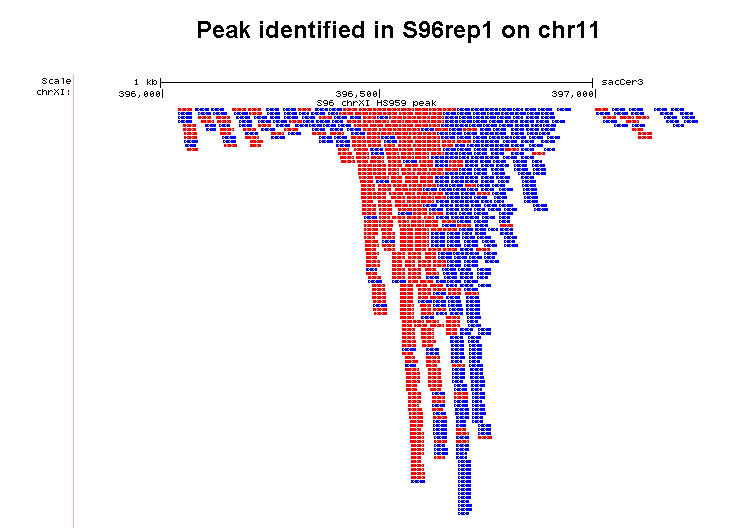
\includegraphics[scale=0.35]{image4_2}

\caption{(left) The correlation score from peaks in HS959 and S96 does not
show a strong positive correlation, with most correlations near zero.
(right) The shared peaks from replicate experiments have more of a
strong positive correlation, with many more peaks showing high positive
correlations.}


\end{figure}


A more recent technique used for finding conserved binding sites using
ChIP-seq is MANorm (Shao et al, 2012). MANorm uses binding sites identified
by a peak finding program and raw ChIP-seq data to fit a linear model
for shared peaks (Figure 3). MA plots use log-product and log-ratio
to compare two experiments, and these techniques have been historically
used for analyzing ChIP-chip arrays but MANorm adapted it to normalize
ChIP-seq data in MANorm. MANorm can also find conserved binding sites
in terms of a Bayesian Poisson model.

\begin{figure}


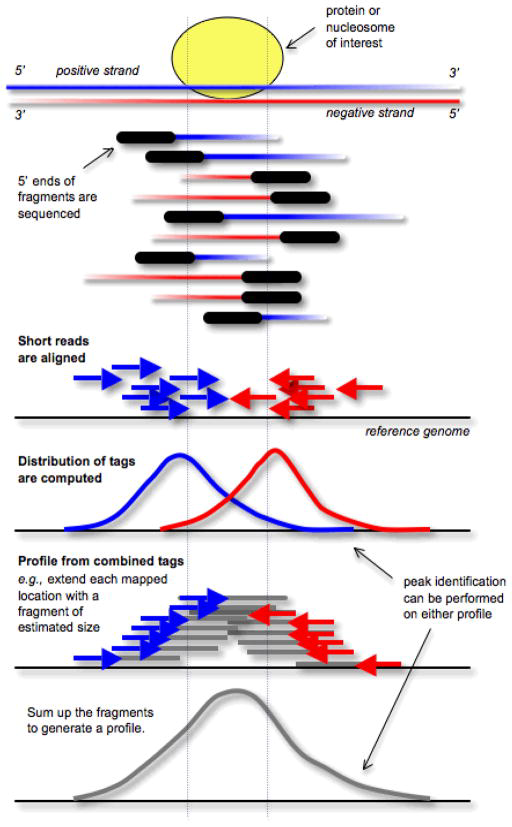
\includegraphics[scale=0.4]{image2}

\caption{MANorm uses the data and peak finding results from two experiments
to normalize the data and to find additional conserved binding sites.}


\end{figure}



\section{Approach}

To determine the scope or the problem of unidentified conserved binding
sites, we calculated the normalized difference score of Zheng et al.
using the number of ChIP-seq tags that overlap each genome position
(see Methods). Then we used a sliding window to calculate the maximum
average NormDiff score for the peaks that are found using MACS as
well as the syntenic region for comparison. We found in many cases
that syntenic regions are enriched with ChIP-seq reads even when it
is not called a binding site by MACS (Figure 4a). To look at both
experiments concurrently, we analyzed a MA plot of the NormDiff scores
that uses the log-product and log-ratio of the maximum average NormDiff
scores overlapping the peaks from both experiments (Figure 4b). The
MA plot shows many binding sites that are unique to one experiment
overlap the same region as the shared binding sites in the figure. 

\begin{figure}
\includegraphics[scale=0.35]{image6_2}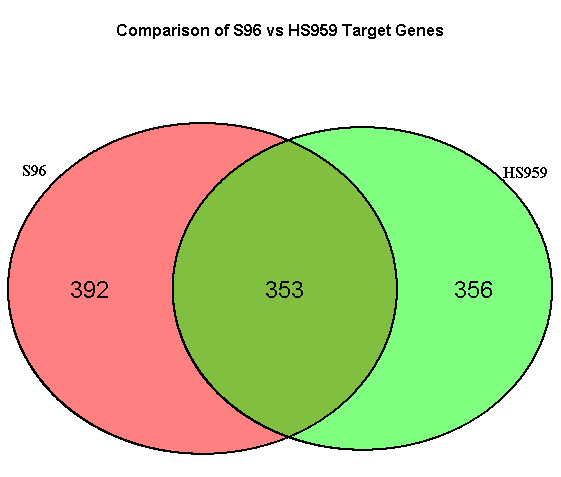
\includegraphics[scale=0.35]{image7_2}

\caption{Comparing the NormDiff score of peaks found using MACS with the syntenic
region of another experiment shows that even sites that aren\textquoteright{}t
called shared have significant NormDiff scores. Note how often there
are red or green points (representing binding sites called in only
one strain) overlapping the region of blue points (which represent
binding sites considered shared by MACS).}


\end{figure}


Peaks that were not identified by MACS but for which there might still
be a shared peak are in what is referred to as the \textquotedblleft{}twilight
zone\textquotedblright{} (Figure 5). Since NormDiff is normalized,
it allows for simple and direct comparison of data. The \textquotedblleft{}twilight
zone\textquotedblright{} represents the overlap of the NormDiff scores
from shared peaks that are at least as big as the syntenic region.
We sorted the the syntenic region\textquoteright{}s max average NormDiff
score for the shared and unique peaks separately (Figure 5). This
shows that some of the strongest NormDiff scores were not called shared
when other weaker signals were called. 

\begin{figure}
\includegraphics[scale=0.35]{image9_2}\includegraphics[scale=0.35]{image10_2}

\caption{The \textquotedblleft{}twilight zone\textquotedblright{} in yellow
shows the NormDiff scores of peaks found to be shared overlap with
NormDiff scores of peaks that were not identified}


\end{figure}



\subsection{Results}

We found 42 new binding sites in HS959 with that were conserved in
S96 that were not identified by MACS with P<0.05, and 4 of binding
sites that were conserved with P<0.01. We also found 76 binding sites
in S96 with P<0.05 that were conserved in HS959, and 13 of these binding
sites were conserved with P<0.01 

To evaluate the significance of these findings, we evaluated all binding
sites from S96 and identified 98\% (885/897) using our method at P<0.05,
and 60\% (563/897) binding sites at a P<0.01. In HS959 we identified
85\% (729/824) of the same binding sites at P<0.05 and 46\% (365/824)
at P<0.01\\


\includegraphics[scale=0.3]{Rplot23}\includegraphics[scale=0.3]{Rplot25_2}\\
Figure 3. The maximum average NormDiff score is used to identify additional
binding sites that are conserved in each experiment. 


\section{Discussion}

Using our method there appeared to be evidence for conserved binding
sites that were not identified by other peak finding algorithms. We
found a significant enrichment of NormDiff scores for many binding
sites, which represents strong binding signals, even for binding sites
that were not identified as shared by MACS. Peaks that were not identified
by MACS but for which there might still be shared peaks, we call the
\textquotedblleft{}twilight zone\textquotedblright{}.\\


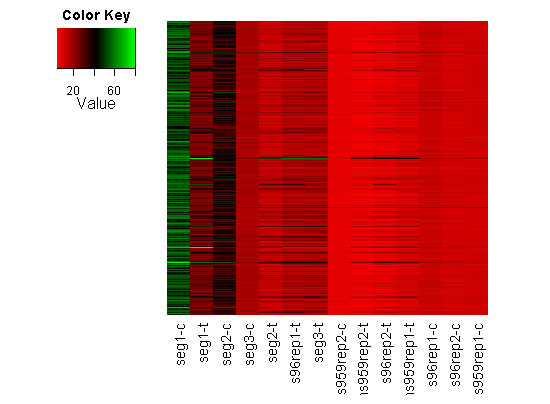
\includegraphics[scale=0.3]{image11}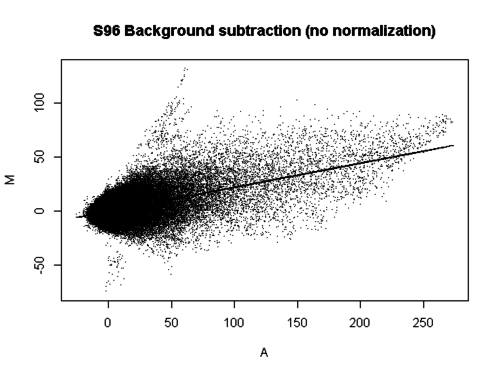
\includegraphics[scale=0.3]{image12}

Figure 4. The twilight zone in yellow shows where the normalized difference
scores from each experiment overlap significantly \\


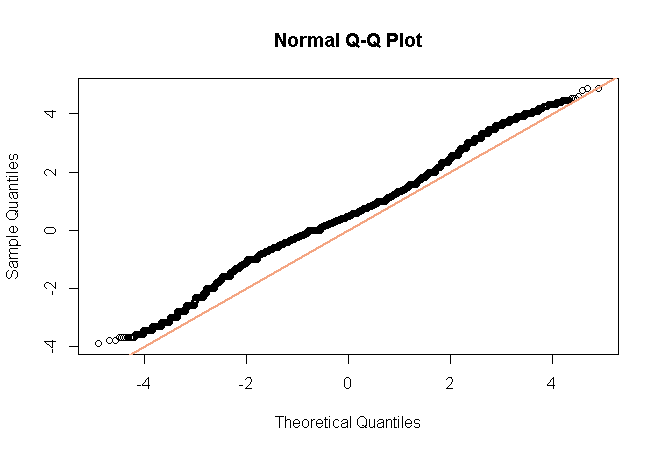
\includegraphics[scale=0.3]{image16}

Figure 5. A shared binding sites that we identified using our algorithm
has the above distribution.\\


Our work could be extended to use more sophisticated statistical models
for NormDiff too. For example, we considered modifying NormDiff scores
to use data from multiple experiments in order to find conserved binding
sites. We also discuss some of the drawbacks of our method, and the
other applications of NormDiff. 


\subsection{Modified normdiff score}

We propose using a modified NormDiff score that uses data from multiple
experiments. A NormDiff score that adds data from two experiments,
A1,B1,A2, and B2 can be defined as \\
\[
Z_{add}(x_{i})=\frac{(A_{1}-B_{1}/c_{1})+(A_{2}-B_{2}/c_{2})}{\sigma}
\]


Then the scaling factors $c_{1}$and $c_{2}$ are estimated from data,
and the variance is $\sigma=\sqrt{A_{1}+B_{1}/c_{1}^{2}+A_{2}+B_{2}/c{}_{2}^{2}}$ 

A NormDiff score that subtracts data from two experiments could also
be defined as
\[
Z_{sub}(x_{i})=\frac{(A_{1}-B_{1}/c_{1})-(A_{2}-B_{2}/c_{2})}{\sigma}
\]


The variance for $Z_{sub}$ would be the same as the variance for
$Z_{add}$. It is possible that adding and subtracting NormDiff scores
might be able to help in identifying conserved and differential binding.
For example, if the subtractive score is small but the additive score
is large, then the binding site is likely to be conserved in both
experiments. This method is similar to an MA plot which compares the
log-product and log-ratio of two experiments, however, our method
does not exaggerate small changes like the log-scale does.\\


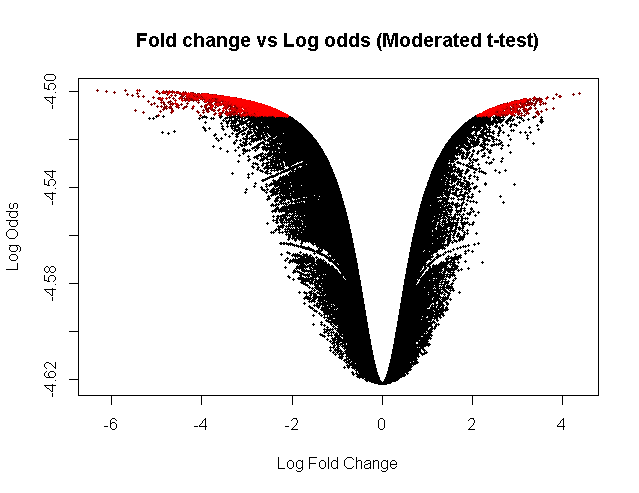
\includegraphics[scale=0.3]{image25}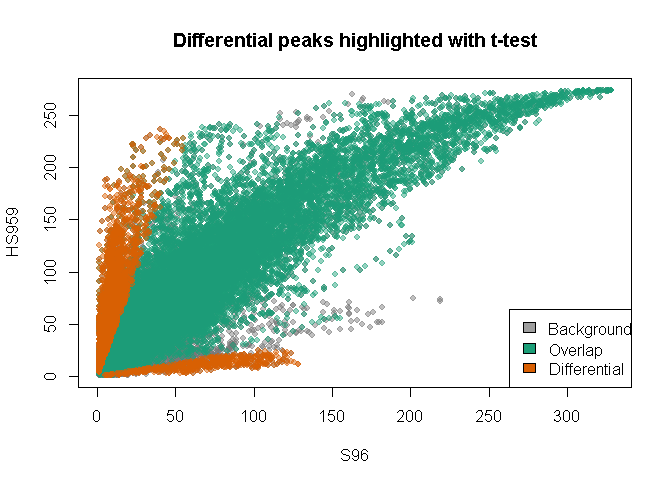
\includegraphics[scale=0.3]{image26}

Figure 6. $Z_{add}$ vs. $Z_{sub}$ for S96 and HS959. The modified
NormDiff scores are used to find evidence of shared binding sites
in the HS959 and S96 genomes. Both genomes are considered concurrently
with the modified NormDiff score to find shared peaks

\includegraphics[scale=0.3]{Rplot05}

Figure 7. MA-plot of shared and unique peaks from S96 and HS959. Unique
peaks to S96 colored green, unique peaks to HS959 colored red, shared
peaks from both colored blue.

.


\subsection{Drawbacks of our approach}

Our approach tries to find evidence for conserved binding sites by
analyzing data using normalized difference scores. Our approach gives
some evidence of peaks with high confidence P-values, such as our
results of finding new peaks with P<0.01. However, these findings
have much less confidence than thresholds set by MACS (P<1e-5). Given
that our technique for calculating P-value is similar to MACS, i.e.
by finding deviations from the background, our results are not very
strong. 

One of the reasons that we have less confidence in P-values is because
NormDiff uses control data for background subtraction. MACS does not
use control data to calculate P-values, but it uses control data to
calculate false discovery rates. Additionally, we use a normal approximation
for our data, but since our data is not continuous it may not behave
as well as Poisson distribution. 


\section{Conclusion}

We found a method for comparing binding sites from different ChIP-seq
experiments by using a normalized difference score. This gave us evidence
for shared binding sites that were not called by other peak finding
algorithms. While it was able to produce some evidence, the confidence
levels were much less than MACS which presented a challenge to the
conclusions we could make. Despite these issues, NormDiff is a powerful
tool for analyzing ChIP-seq data in other ways. NormDiff effectively
models the ChIP-seq binding signal and it can be used to compare ChIP-seq
data across multiple experiments


\section{Methods}


\subsection{Normalized difference scores}

The normalized difference (NormDiff) score is a useful statistic for
comparing ChIP-seq data that uses background subtraction and normalization
to obtain the ChIP-seq binding signal. The NormDiff score from Zheng
et al. uses a simple random model for ChIP-seq ($A$) and control
($B$) defined as

\begin{eqnarray*}
A & \sim & Poisson(f+g)\\
B & \sim & Poisson(cg)
\end{eqnarray*}


Where- 

$f$ represents the binding signal

$g$ represents the background noise

$c$ is a scaling factor between $A$ and $B$\\


Then, the NormDiff $Z$ is defined for each genome position $x_{i}$
as 

\[
Z(x_{i})=\frac{A(x_{i})-B(x_{i})/c}{\sigma}
\]
 

Then the scaling factor $c$ is estimated as the median ratio of $A/B$
and the variance $\sigma$ is estimated from $\sqrt{A+B/c^{2}}$.\\


\includegraphics[scale=0.3]{Rplot08}\includegraphics[scale=0.3]{Rplot05_2}

Supplemental Figure 1. (left) Kernel density plot of NormDiff for
entire genome shows approximately normal distribution. (right) Q-Q
Plot shows that the binding signal deviates significantly from the
expected normal distribution.


\section{Bibliography}

\bibliographystyle{plain}
\nocite{*}
\bibliography{References}

\end{document}
